\chapter{Конструкторский раздел}
В данном разделе выполнено проектирование программное обеспечения.

\section{Определение прецедентов}
Для того, чтобы рекомендательная система удовлетворяла требованиям, сформулированным на этапе анализа, необходимо выделить минимальный набор прецедентов.
К необходимым прецедентам относятся:
\begin{itemize}
	\item получение рекомендаций рецепта по введённому набору продуктов;
	\item присвоить рецепту оценку от $1$ до $5$;
	\item изменить оценку рецепта;
	\item удалить оценку рецепта;
	\item получить список оценок пользователя;
	\item поиск рецепта по локальной базе данных;
	\item создать аккаунт для синхронизации данных на различных устройствах;
	\item войти в аккаунт.
\end{itemize}

Также предусмотрены популярные дополнительные прецеденты, повышающие удобство использования приложения~\cite{app_foodru}.
Далее представлен их список:
\begin{itemize}
	\item выйти из аккаунта;
	\item удалить рецепт из избранного;
	\item добавить рецепт в избранное;
	\item получить избранные рецепты.
\end{itemize}

В результате получается диаграмма прецедентов, показанная на рисунке~\ref{fig:usecases}.
\begin{figure}[H]
	\centering
	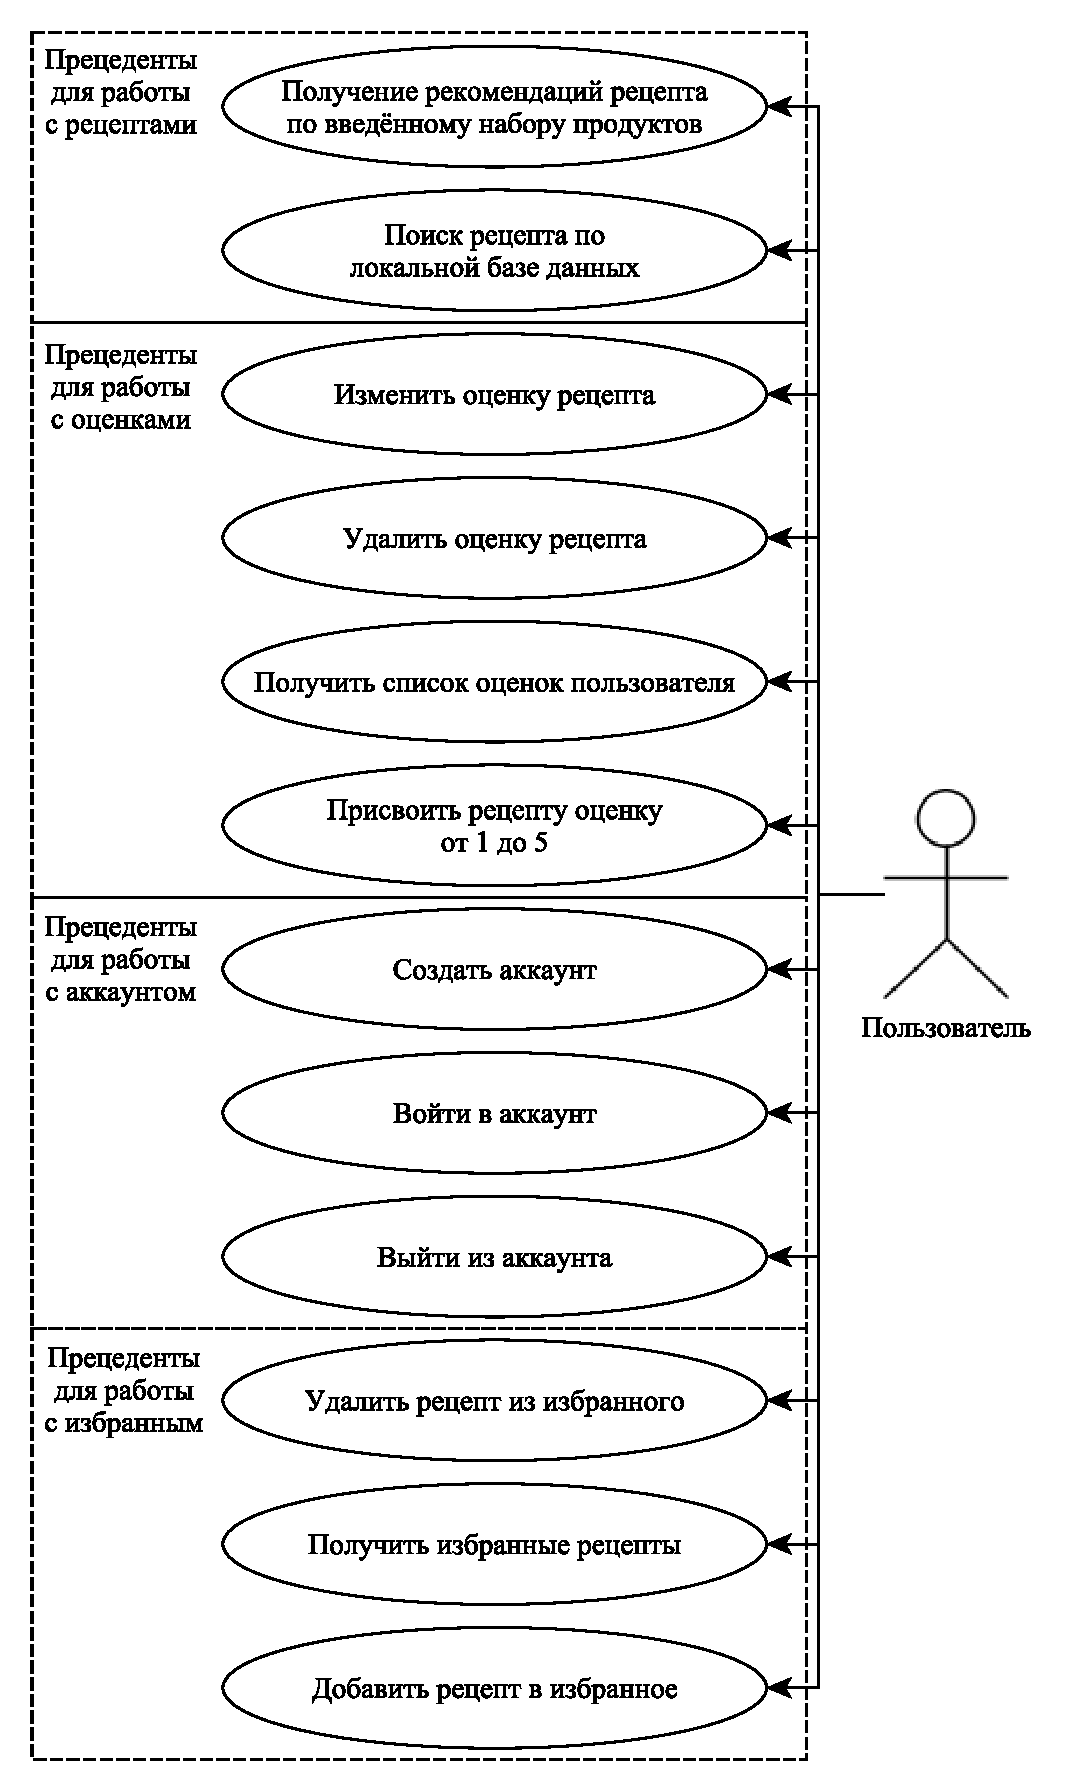
\includegraphics[height=0.85\textheight]{img/usecases.pdf}
	\caption{
	    Диаграмма прецедентов рекомендательной системы
	}
	\label{fig:usecases}
\end{figure}

\section{Выделение сущностей}
В приложении данные представляются в виде сущностей.
На рисунке~\ref{fig:er} представлена диаграмма сущность-связь для всей рекомендательной системы.
Сущность тега представляет собой характеристику рецепта, по которой их можно фильтровать.
Таким образом, пользователь имеет больше контроля над результатами рекомендаций.
\begin{figure}[H]
	\centering
	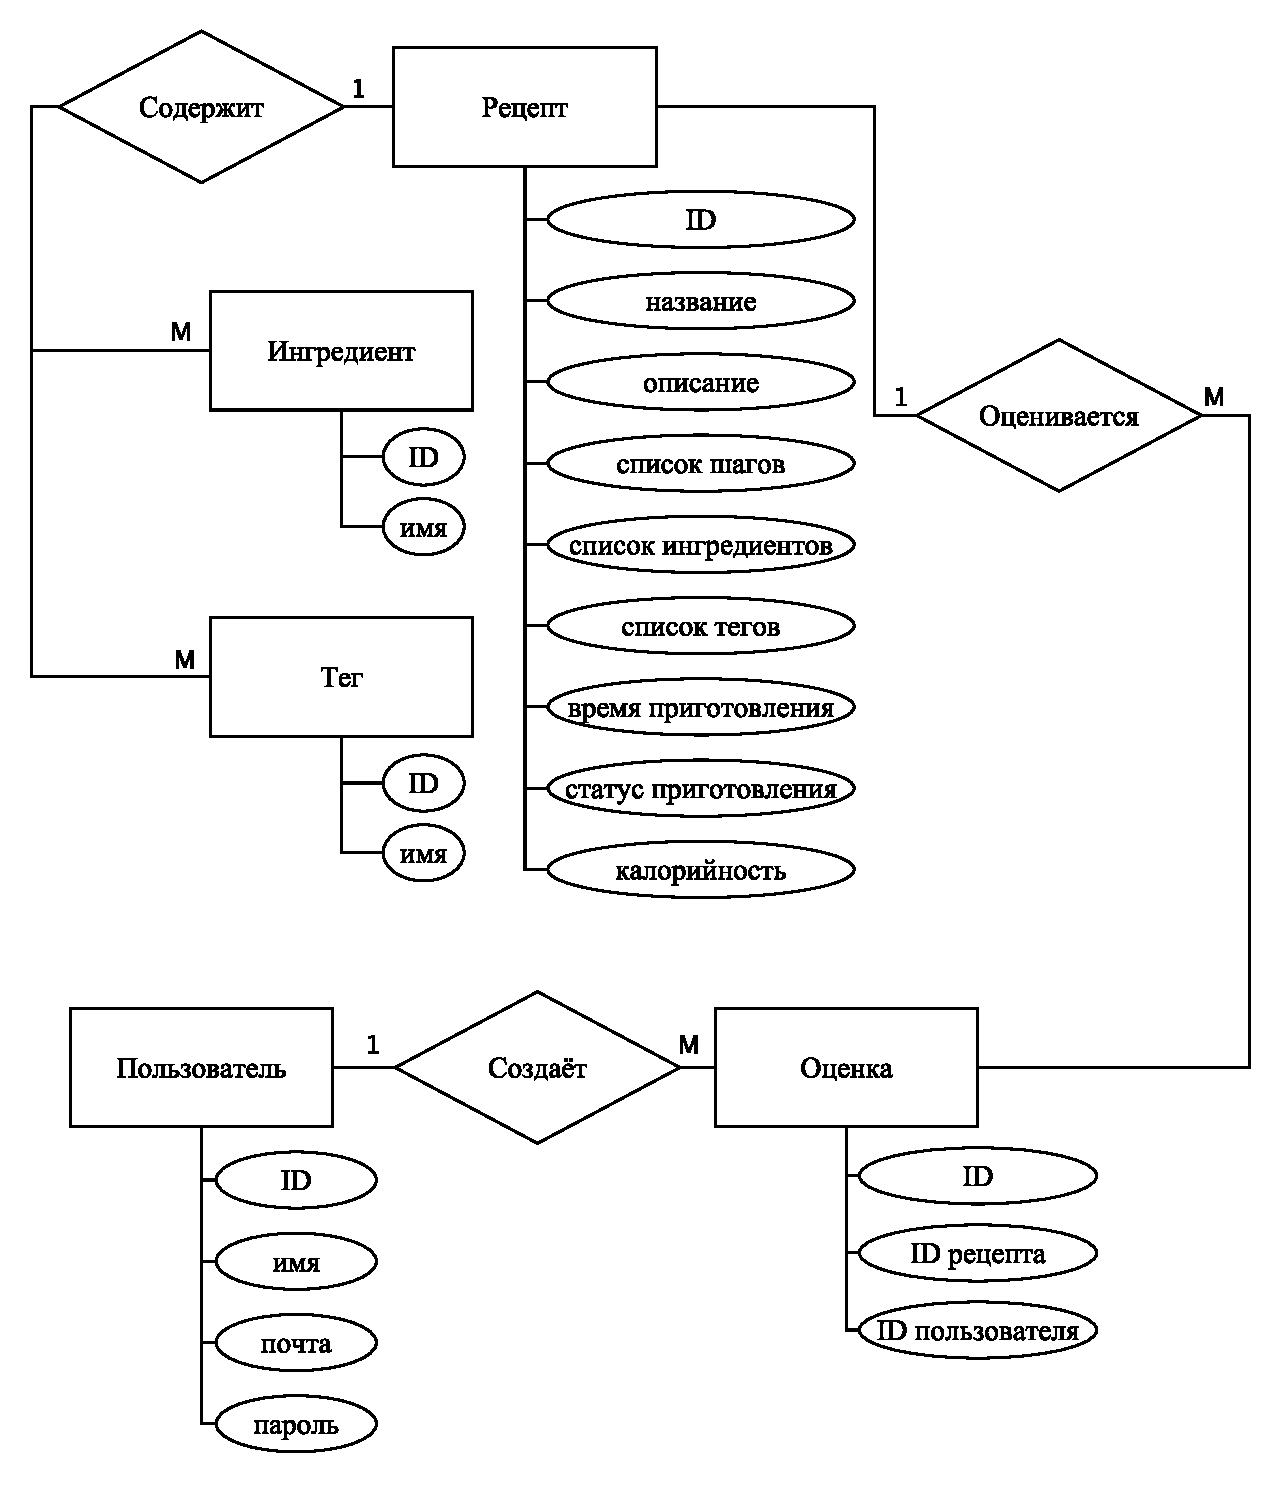
\includegraphics[width=0.95\textwidth]{img/er.pdf}
	\caption{
	    Схема сущность-связь для разрабатываемой рекомендательной системы
	}
	\label{fig:er}
\end{figure}
В системе локально хранятся следующие сущности:
\begin{itemize}
	\item рецепт;
	\item ингредиент рецепта;
	\item тег рецепта.
\end{itemize}
Такие сущности как пользователь и оценка должны храниться удалённо, чтобы обеспечить пользователю автоматически копировать оценки рецептов на другие устройства.

\section{Выбор архитектурных шаблонов проектирования}
Необходимо определить общие правила функционирования разрабатываемого программного обеспечения.
Это делается с помощью выбора архитектурных шаблонов проектирования.
Для связи между пользователем и прецедентами был выбран шаблон <<Model-View-Intent>>~\cite{arkivanov}.
Также для разработки выбраны принципы чистой архитектуры, так как они позволяют легче переносить приложение между операционными системами~\cite{robert_martin}.
На рисунке~\ref{fig:mvi} представлена схема взаимодействия пользователя с прецедентами, а рисунок~\ref{fig:uml} отображает UML-диаграмму компонентов приложения в соответствии с чистой архитектурой.
\begin{figure}[h]
	\centering
	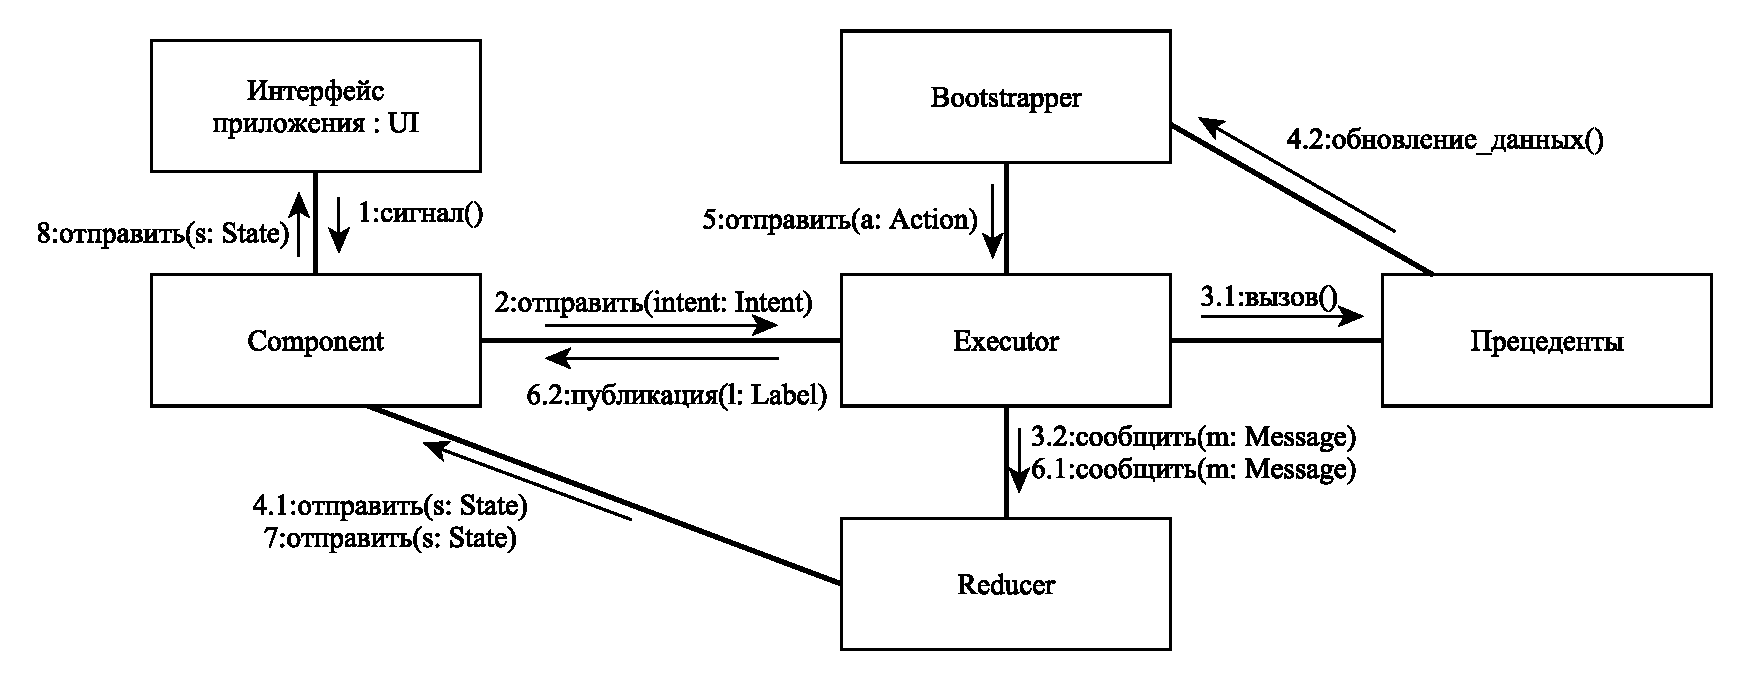
\includegraphics[width=\textwidth]{img/mvi.pdf}
	\caption{
	    Коммуникационная диаграмма, отражающая принцип работы архитектурного шаблона проектирования MVI
	}
	\label{fig:mvi}
\end{figure}

\begin{figure}[h]
	\centering
	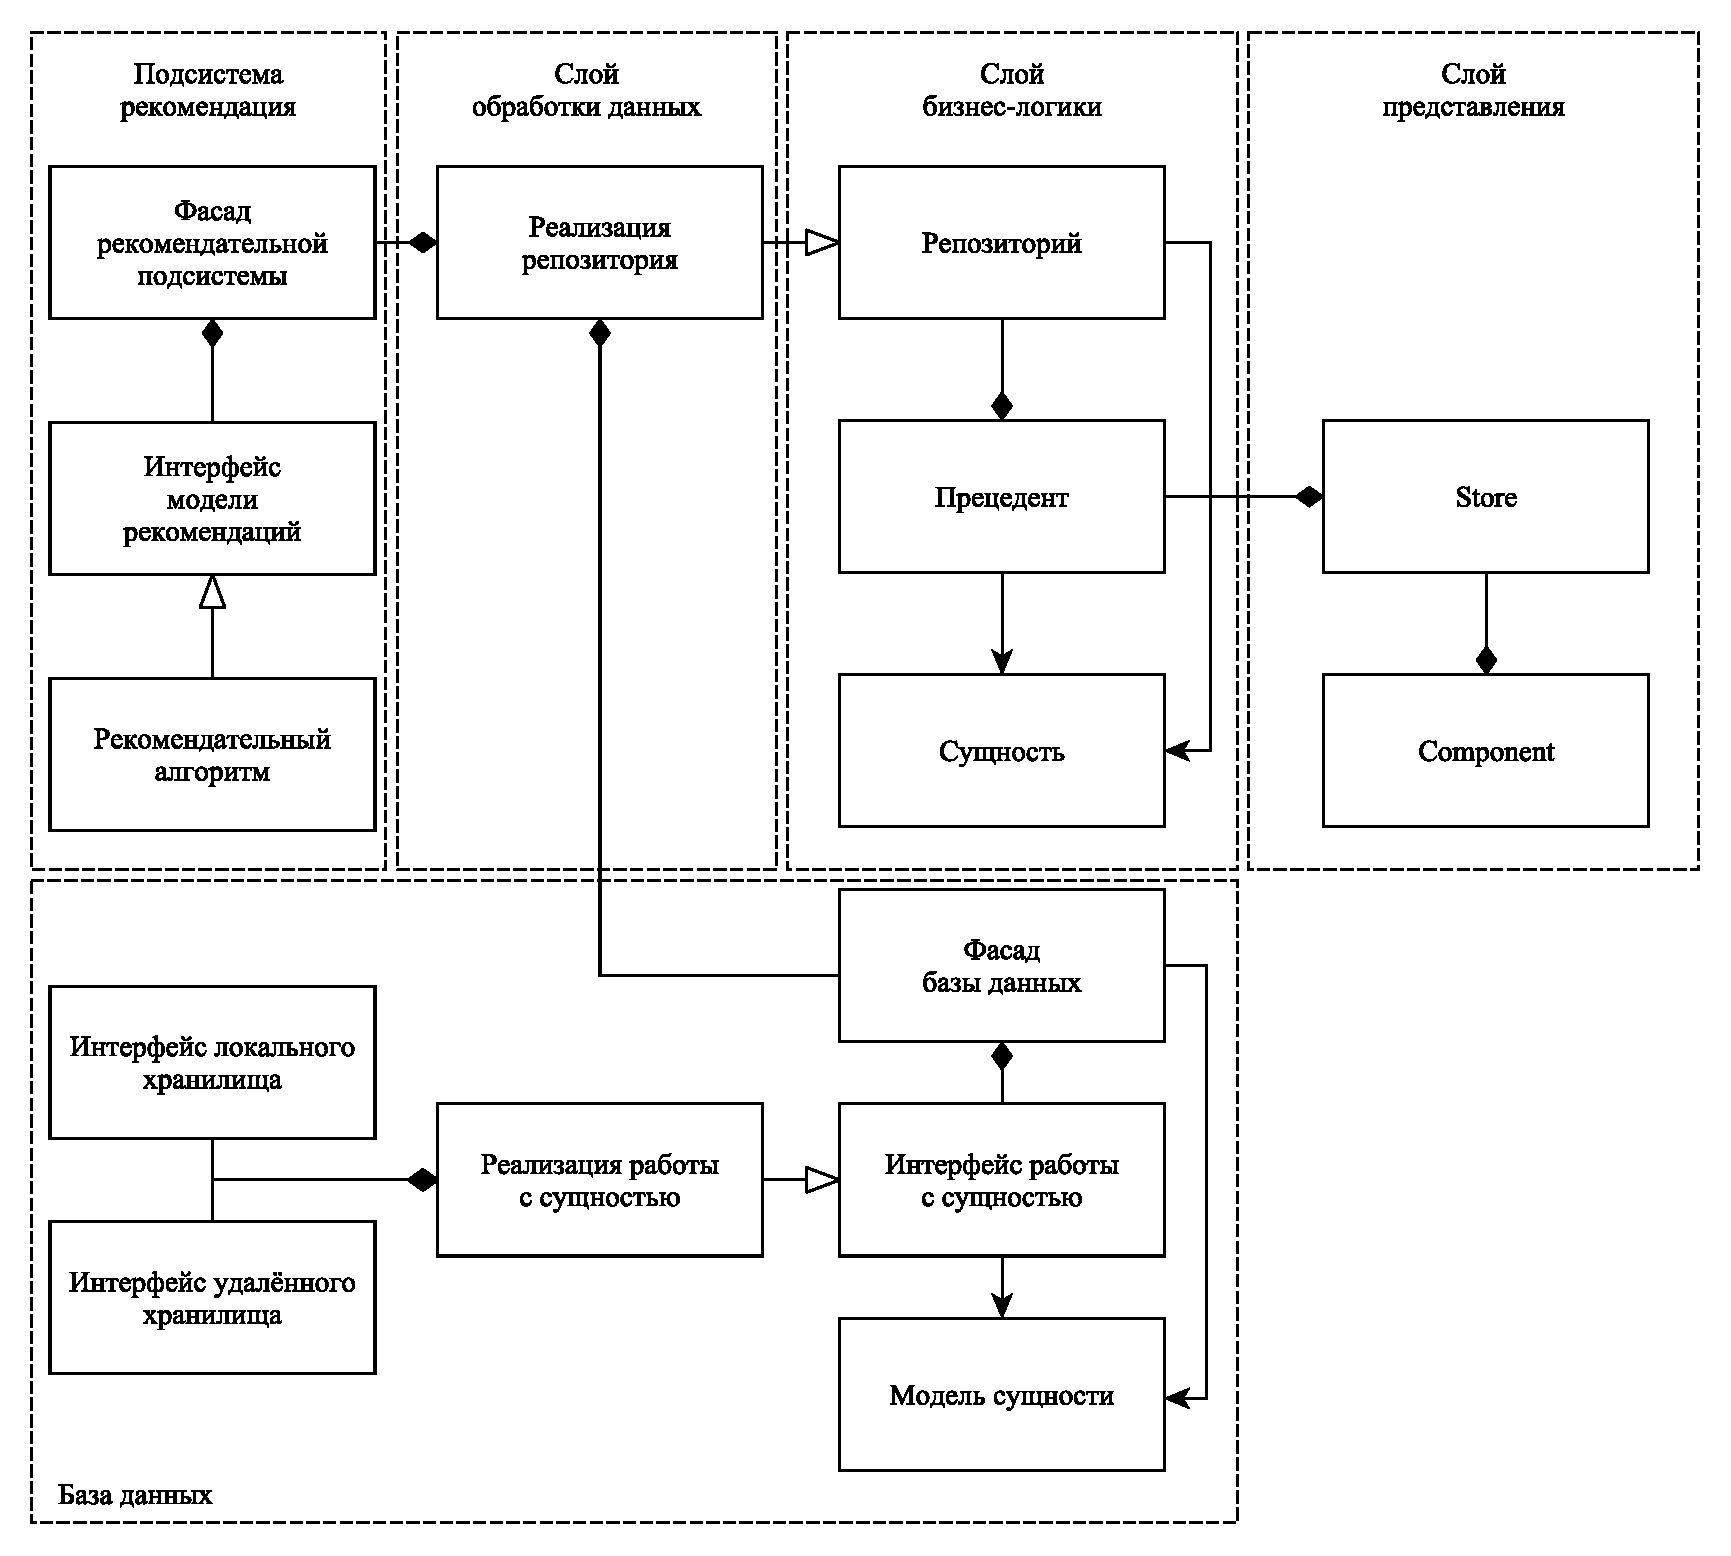
\includegraphics[width=\textwidth]{img/uml.pdf}
	\caption{
	    UML-диаграмма компонентов приложения и зависимостей между ними в соответствии с <<чистой архитектурой>>
	}
	\label{fig:uml}
\end{figure}

\section{Проектирование алгоритма рекомендаций}
Основные этапы работы подсистемы рекомендаций представлены на рисункaх~\ref{fig:idef0}--\ref{fig:idef3} в виде IDEF0 диаграмм.
\begin{figure}[htbp]
	\centering
	\imgfig{img/idef0}
	\caption{
	    IDEF0 диаграмма уровня 0 работы рекомендательной подсистемы
	}
	\label{fig:idef0}
\end{figure}
\begin{figure}[htbp]
	\centering
	\imgfig{img/idef1}
	\caption{
	    IDEF0 диаграмма уровня 1 работы рекомендательной подсистемы
	}
	\label{fig:idef1}
\end{figure}
\begin{figure}[htbp]
	\centering
	\imgfig{img/idef2}
	\caption{
	    IDEF0 диаграмма уровня 2 работы рекомендательной подсистемы
	}
	\label{fig:idef2}
\end{figure}
\begin{figure}[htbp]
	\centering
	\imgfig{img/idef3}
	\caption{
	    IDEF0 диаграмма уровня 3 работы рекомендательной подсистемы
	}
	\label{fig:idef3}
\end{figure}

Далее на рисунках~\ref{fig:profile}--\ref{fig:filter} изображены схемы алгоритмов, декомпозирующих блоки IDEF0 диаграммы.
\begin{figure}[htbp]
	\centering
	\imgfig{img/profile}
	\caption{
	    Схема алгоритма построения профиля пользователя, декомпозирующая блок 2.2.1 на диаграмме~\ref{fig:idef3}
	}
	\label{fig:profile}
\end{figure}
\begin{figure}[h]
	\centering
	\imgfig{img/metrics}
	\caption{
	    Схема алгоритма вычисления метрик, декомпозирующая блок 2.2.2 на диаграмме~\ref{fig:idef3}, результатом работы являются параметры рекомендательной модели
	}
	\label{fig:metrics}
\end{figure}
\begin{figure}[htbp]
	\centering
	\imgfig{img/learn}
	\caption{
	    Схема алгоритма обучения регрессии, декомпозирующая блок 2.2.3 на диаграмме~\ref{fig:idef3}
	}
	\label{fig:learn}
\end{figure}
\begin{figure}[htbp]
	\centering
	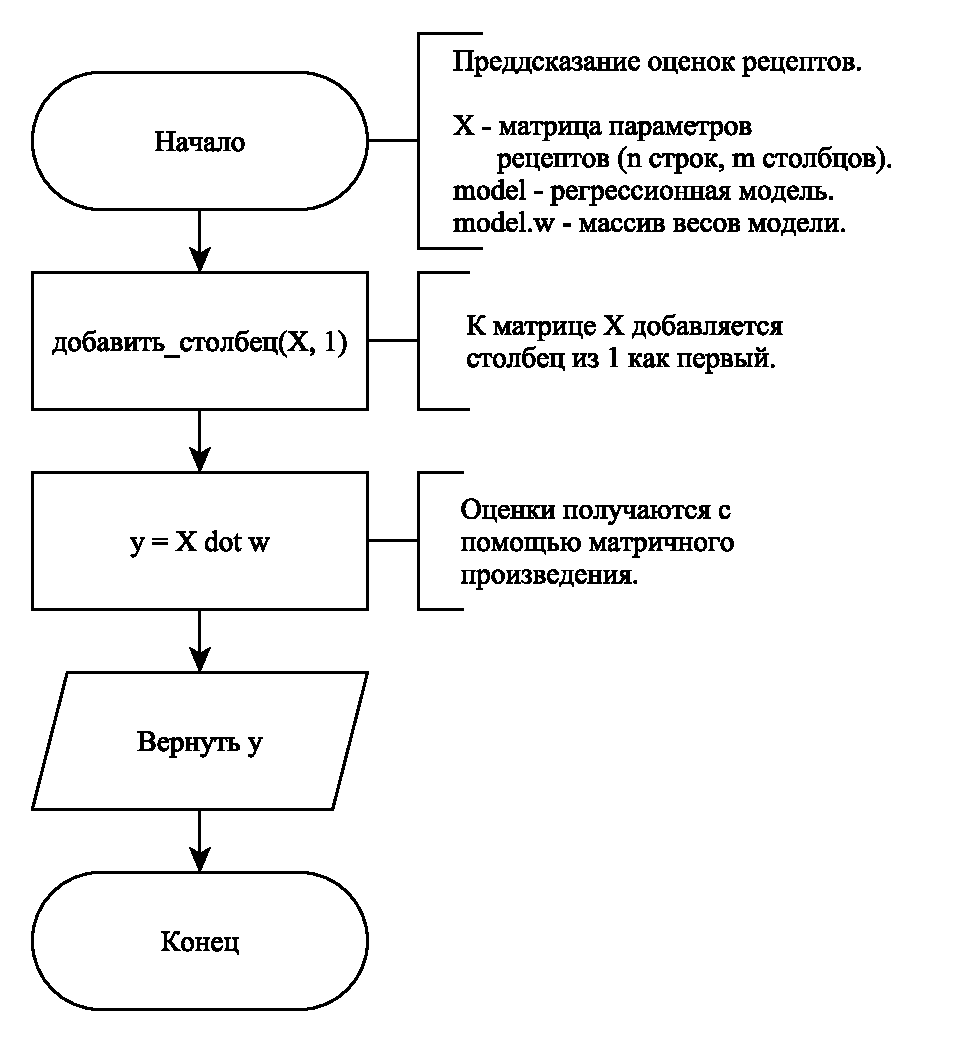
\includegraphics[height=0.3\textheight]{img/predict.pdf}
	\caption{
	    Схема алгоритма предсказания оценок, декомпозирующая блок 2.3 на диаграмме~\ref{fig:idef3}
	}
	\label{fig:predict}
\end{figure}
\begin{figure}[htbp]
	\centering
	\imgfig{img/assemble}
	\caption{
	    Схема алгоритма формирования списка рецептов, декомпозирующая блок 3 на диаграмме~\ref{fig:idef1}
	}
	\label{fig:assemble}
\end{figure}
\begin{figure}[htbp]
	\centering
	\imgfig{img/filter}
	\caption{
	    Схема алгоритма фильтрации списка рецептов, декомпозирующая блок 4 на диаграмме~\ref{fig:idef1}
	}
	\label{fig:filter}
\end{figure}

\section*{Вывод из конструкторского раздела}
В результате данного раздела выделены прецеденты рекомендательной системы, проведено проектирование алгоритма её работы, и произведён выбор архитектурных шаблонов проектирования.
Таким образом, получены все необходимые сведения для реализации программного обеспечения.

